\documentclass[12pt]{article} %Tipo de documento

\usepackage[utf8]{inputenc}	%Codificación
\usepackage[spanish]{babel} %Idioma
\usepackage{fancyhdr, graphicx, parskip}
\usepackage[margin=1in]{geometry} %para el identado de párrafos
\usepackage{indentfirst}%para el identado de párrafos
\usepackage{array}%Tamaño de celdas
\usepackage{blindtext}%Enumeraciones
\usepackage{xcolor}
\usepackage{hyperref} %enlaces
\usepackage{colortbl} %Color de las tablas
\usepackage{lscape} %Hojas en horizontal

\graphicspath{ {images/} } %Para las imagenes del fancyhead
\renewcommand{\headrulewidth}{0pt}
\pagestyle{empty}


\fancyhead[L]{
	
\includegraphics[width=2cm]{unam.jpg}
}
\fancyhead[R]{
	
\includegraphics[width=2cm]{FI.jpg}
}
\fancyfoot[C]{}

\title{Propuesta de proyecto final}
\author{Gabriel Rojas, Max Schouten, Fernanda Jiménez}
\date{\today}

\begin{document}
	%Portada
	\begin{titlepage}
		\thispagestyle{fancy}
		\centering
		{\bfseries - \par}
		\vspace{0.7cm}
		{\bfseries\LARGE UNIVERSIDAD NACIONAL AUTÓNOMA DE MÉXICO \par}
		\vspace{0.7cm}
		{\bfseries\LARGE Facultad de Ingeniería \par}
		\vspace{1cm}
		{\bfseries\LARGE Computación Gráfica e Interacción Humano Computadora \par}
		\vspace{0.5cm}
		{\bfseries\LARGE Ing. José Roque Román Guadarrama \par}
		\vspace{0.5cm}
		{\bfseries\LARGE Croquis del proyecto final \par}
		\vspace{0.5cm}
		{\bfseries\LARGE Cruz Schouten Max Bernardo \par}
		{\bfseries\Large No. Cuenta: 314081205 | Teoría: 01\par}
		{\bfseries\LARGE Jiménez García Fernanda \par}
		{\bfseries\Large No. Cuenta: 314081205 | Teoría: 01\par}
		{\bfseries\LARGE Rojas Méndez Gabriel \par}
		{\bfseries\Large No. Cuenta: 314141712 | teoría: 01\par}
		\vspace{1cm}
		{\bfseries\LARGE Fecha de entrega: 27 de marzo de 2020 \par}
		\vspace{1cm}
		{\bfseries\LARGE Semestre 2020-2 \par}
	\end{titlepage}
	
	\newpage
		\section{Croquis}
		\setlength{\parindent}{1.0cm}
		El boceto del zoológico se pretende diseñar de la siguiente manera, en donde se tienen elementos como agua, árboles, los dinosaurios, un helicóptero y el avatar principal que será el personaje de Bender de la serie animada de Futurama. 
		\setlength{\parindent}{0.0cm}
		\begin{figure}[h]
			\begin{center}
				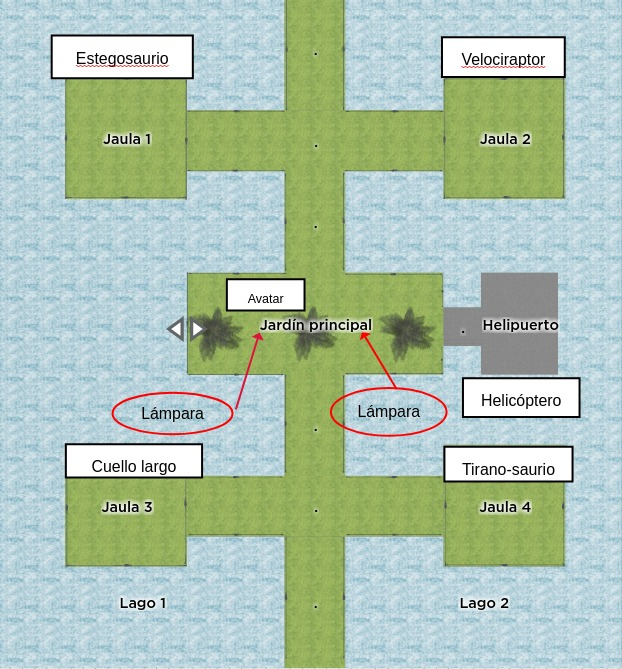
\includegraphics[scale=0.9]{images/Plano.png}
				\caption{Distribución de los elementos}
			\end{center}		
		\end{figure}
	
		\newpage
		\begin{landscape}
		\setlength{\parindent}{1.0cm}
		La vista en plano del suelo se pretende que sea como la siguiente, aunque aquí no se logran apreciar los elementos ya mencionados por limitaciones de \color{blue}\url{https://home.by.me/es/mis-proyectos}\color{black} pero ya están detalladas en el boceto de vista superior.
		\setlength{\parindent}{0.0cm}
		\begin{figure}[h]
			\begin{center}
				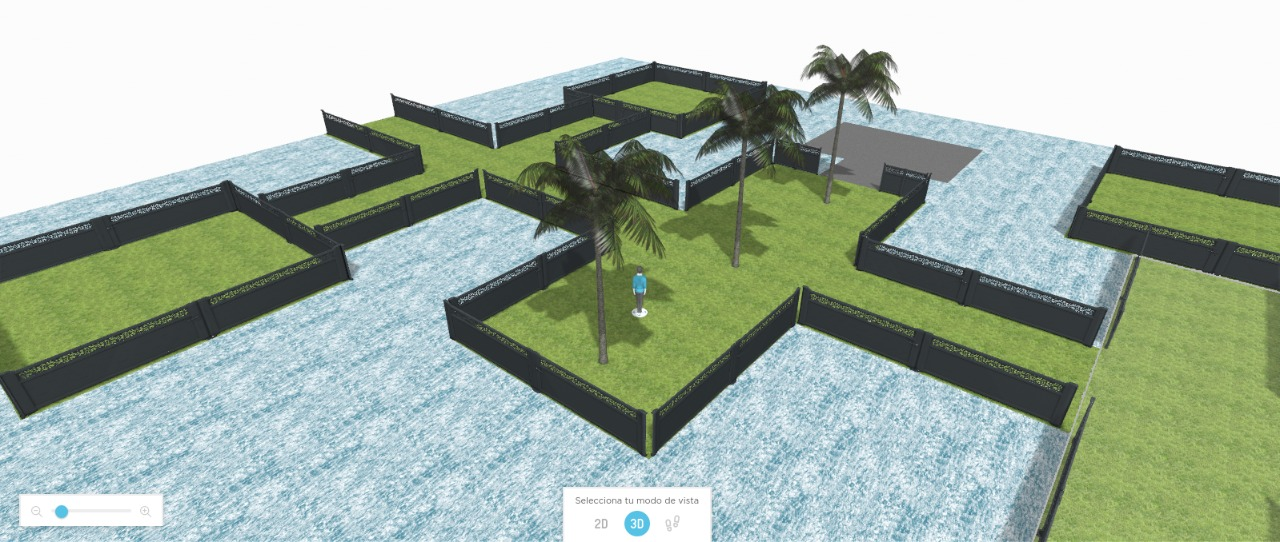
\includegraphics[scale=0.8]{images/vista.png}
				\caption{Distribución de los elementos}
			\end{center}		
		\end{figure}
	\end{landscape}
\end{document}